\documentclass{standalone}
\usepackage{tikz}
\usetikzlibrary{patterns, positioning}

\begin{document}
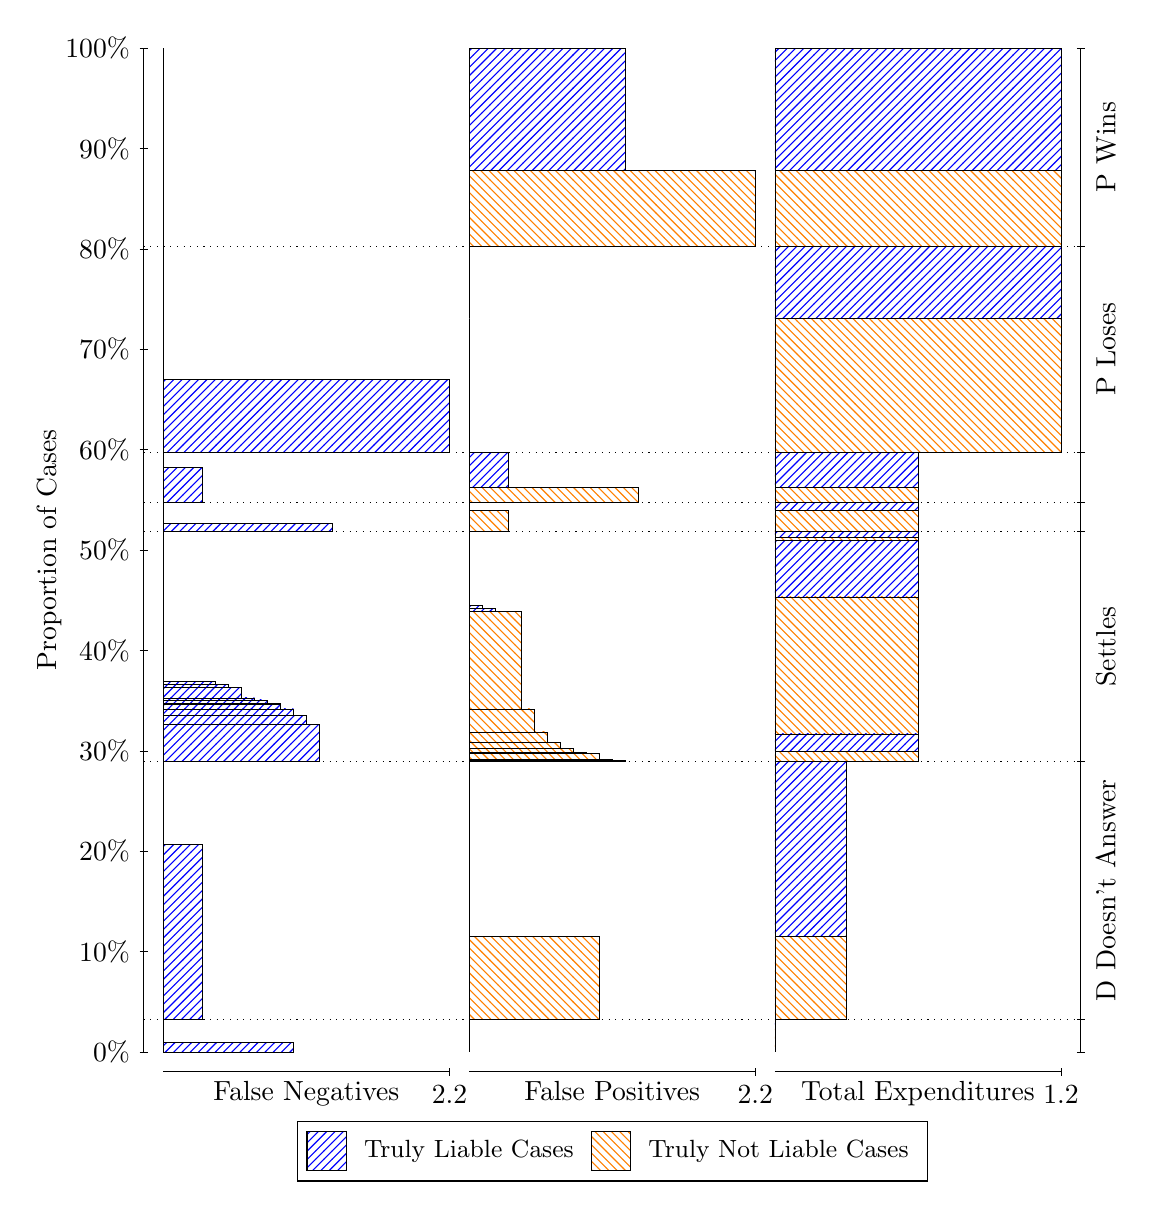
\begin{tikzpicture}
\draw[black, very thin] (1.5,1.75) -- (1.5,14.5);
\node[rotate=90, anchor=center] at (0.3, 8.125) {Proportion of Cases};
\draw[black, very thin] (1.45,1.75) -- (1.55,1.75);
\node[anchor=east] at (1.45, 1.75) {0\%};
\draw[black, very thin] (1.45,3.025) -- (1.55,3.025);
\node[anchor=east] at (1.45, 3.025) {10\%};
\draw[black, very thin] (1.45,4.3) -- (1.55,4.3);
\node[anchor=east] at (1.45, 4.3) {20\%};
\draw[black, very thin] (1.45,5.575) -- (1.55,5.575);
\node[anchor=east] at (1.45, 5.575) {30\%};
\draw[black, very thin] (1.45,6.85) -- (1.55,6.85);
\node[anchor=east] at (1.45, 6.85) {40\%};
\draw[black, very thin] (1.45,8.125) -- (1.55,8.125);
\node[anchor=east] at (1.45, 8.125) {50\%};
\draw[black, very thin] (1.45,9.4) -- (1.55,9.4);
\node[anchor=east] at (1.45, 9.4) {60\%};
\draw[black, very thin] (1.45,10.675) -- (1.55,10.675);
\node[anchor=east] at (1.45, 10.675) {70\%};
\draw[black, very thin] (1.45,11.95) -- (1.55,11.95);
\node[anchor=east] at (1.45, 11.95) {80\%};
\draw[black, very thin] (1.45,13.225) -- (1.55,13.225);
\node[anchor=east] at (1.45, 13.225) {90\%};
\draw[black, very thin] (1.45,14.5) -- (1.55,14.5);
\node[anchor=east] at (1.45, 14.5) {100\%};

\draw[black, very thin] (13.4,1.75) -- (13.4,14.5);
\draw[black, very thin] (13.35,1.75) -- (13.45,1.75);
\node[anchor=west] at (13.35, 1.75) {};
\draw[black, very thin] (13.35,2.1607) -- (13.45,2.1607);
\node[anchor=west] at (13.35, 2.1607) {};
\draw[black, very thin] (13.35,5.4429) -- (13.45,5.4429);
\node[anchor=west] at (13.35, 5.4429) {};
\draw[black, very thin] (13.35,8.3575) -- (13.45,8.3575);
\node[anchor=west] at (13.35, 8.3575) {};
\draw[black, very thin] (13.35,8.7325) -- (13.45,8.7325);
\node[anchor=west] at (13.35, 8.7325) {};
\draw[black, very thin] (13.35,9.3687) -- (13.45,9.3687);
\node[anchor=west] at (13.35, 9.3687) {};
\draw[black, very thin] (13.35,11.983) -- (13.45,11.983);
\node[anchor=west] at (13.35, 11.983) {};
\draw[black, very thin] (13.35,14.5) -- (13.45,14.5);
\node[anchor=west] at (13.35, 14.5) {};

\draw[black, very thin, pattern color=blue, pattern=north east lines] (1.75,1.75) rectangle (3.4015,1.8682);
\draw[black, very thin, pattern color=orange, pattern=north west lines] (1.75,1.8682) rectangle (1.75,2.1607);
\draw[black, very thin, pattern color=blue, pattern=north east lines] (1.75,2.1607) rectangle (2.2455,4.3876);
\draw[black, very thin, pattern color=orange, pattern=north west lines] (1.75,4.3876) rectangle (1.75,5.4429);
\draw[black, very thin, pattern color=blue, pattern=north east lines] (1.75,5.4429) rectangle (3.7318,5.9067);
\draw[black, very thin, pattern color=blue, pattern=north east lines] (1.75,5.9067) rectangle (3.5667,6.0272);
\draw[black, very thin, pattern color=blue, pattern=north east lines] (1.75,6.0272) rectangle (3.4015,6.1077);
\draw[black, very thin, pattern color=blue, pattern=north east lines] (1.75,6.1077) rectangle (3.2364,6.1627);
\draw[black, very thin, pattern color=blue, pattern=north east lines] (1.75,6.1627) rectangle (3.2364,6.1721);
\draw[black, very thin, pattern color=blue, pattern=north east lines] (1.75,6.1721) rectangle (3.0712,6.2224);
\draw[black, very thin, pattern color=blue, pattern=north east lines] (1.75,6.2224) rectangle (2.9061,6.2471);
\draw[black, very thin, pattern color=blue, pattern=north east lines] (1.75,6.2471) rectangle (2.7409,6.3793);
\draw[black, very thin, pattern color=blue, pattern=north east lines] (1.75,6.3793) rectangle (2.5758,6.4142);
\draw[black, very thin, pattern color=blue, pattern=north east lines] (1.75,6.4142) rectangle (2.4106,6.4534);
\draw[black, very thin, pattern color=orange, pattern=north west lines] (1.75,6.4534) rectangle (1.75,8.3575);
\draw[black, very thin, pattern color=blue, pattern=north east lines] (1.75,8.3575) rectangle (3.897,8.4621);
\draw[black, very thin, pattern color=orange, pattern=north west lines] (1.75,8.4621) rectangle (1.75,8.7325);
\draw[black, very thin, pattern color=blue, pattern=north east lines] (1.75,8.7325) rectangle (2.2455,9.1763);
\draw[black, very thin, pattern color=orange, pattern=north west lines] (1.75,9.1763) rectangle (1.75,9.3687);
\draw[black, very thin, pattern color=blue, pattern=north east lines] (1.75,9.3687) rectangle (5.3833,10.289);
\draw[black, very thin, pattern color=orange, pattern=north west lines] (1.75,10.289) rectangle (1.75,11.983);
\draw[black, very thin, pattern color=orange, pattern=north west lines] (1.75,11.983) rectangle (1.75,12.95);
\draw[black, very thin, pattern color=blue, pattern=north east lines] (1.75,12.95) rectangle (1.75,14.5);
\draw[black, very thin, pattern color=orange, pattern=north west lines] (5.6333,1.75) rectangle (5.6333,2.0426);
\draw[black, very thin, pattern color=blue, pattern=north east lines] (5.6333,2.0426) rectangle (5.6333,2.1607);
\draw[black, very thin, pattern color=orange, pattern=north west lines] (5.6333,2.1607) rectangle (7.2848,3.2161);
\draw[black, very thin, pattern color=blue, pattern=north east lines] (5.6333,3.2161) rectangle (5.6333,5.4429);
\draw[black, very thin, pattern color=orange, pattern=north west lines] (5.6333,5.4429) rectangle (7.6152,5.4553);
\draw[black, very thin, pattern color=orange, pattern=north west lines] (5.6333,5.4553) rectangle (7.45,5.4679);
\draw[black, very thin, pattern color=orange, pattern=north west lines] (5.6333,5.4679) rectangle (7.2848,5.5383);
\draw[black, very thin, pattern color=orange, pattern=north west lines] (5.6333,5.5383) rectangle (7.1197,5.5551);
\draw[black, very thin, pattern color=orange, pattern=north west lines] (5.6333,5.5551) rectangle (6.9545,5.6009);
\draw[black, very thin, pattern color=orange, pattern=north west lines] (5.6333,5.6009) rectangle (6.7894,5.6823);
\draw[black, very thin, pattern color=orange, pattern=north west lines] (5.6333,5.6823) rectangle (6.6242,5.8141);
\draw[black, very thin, pattern color=orange, pattern=north west lines] (5.6333,5.8141) rectangle (6.4591,6.1074);
\draw[black, very thin, pattern color=orange, pattern=north west lines] (5.6333,6.1074) rectangle (6.2939,7.347);
\draw[black, very thin, pattern color=blue, pattern=north east lines] (5.6333,7.347) rectangle (5.9636,7.3863);
\draw[black, very thin, pattern color=blue, pattern=north east lines] (5.6333,7.3863) rectangle (5.7985,7.4212);
\draw[black, very thin, pattern color=blue, pattern=north east lines] (5.6333,7.4212) rectangle (5.6333,8.3575);
\draw[black, very thin, pattern color=orange, pattern=north west lines] (5.6333,8.3575) rectangle (6.1288,8.6278);
\draw[black, very thin, pattern color=blue, pattern=north east lines] (5.6333,8.6278) rectangle (5.6333,8.7325);
\draw[black, very thin, pattern color=orange, pattern=north west lines] (5.6333,8.7325) rectangle (7.7803,8.9249);
\draw[black, very thin, pattern color=blue, pattern=north east lines] (5.6333,8.9249) rectangle (6.1288,9.3687);
\draw[black, very thin, pattern color=orange, pattern=north west lines] (5.6333,9.3687) rectangle (5.6333,11.062);
\draw[black, very thin, pattern color=blue, pattern=north east lines] (5.6333,11.062) rectangle (5.6333,11.983);
\draw[black, very thin, pattern color=orange, pattern=north west lines] (5.6333,11.983) rectangle (9.2667,12.95);
\draw[black, very thin, pattern color=blue, pattern=north east lines] (5.6333,12.95) rectangle (7.6152,14.5);
\draw[black, very thin, pattern color=orange, pattern=north west lines] (9.5167,1.75) rectangle (9.5167,2.0426);
\draw[black, very thin, pattern color=blue, pattern=north east lines] (9.5167,2.0426) rectangle (9.5167,2.1607);
\draw[black, very thin, pattern color=orange, pattern=north west lines] (9.5167,2.1607) rectangle (10.425,3.2161);
\draw[black, very thin, pattern color=blue, pattern=north east lines] (9.5167,3.2161) rectangle (10.425,5.4429);
\draw[black, very thin, pattern color=orange, pattern=north west lines] (9.5167,5.4429) rectangle (11.333,5.5718);
\draw[black, very thin, pattern color=blue, pattern=north east lines] (9.5167,5.5718) rectangle (11.333,5.7891);
\draw[black, very thin, pattern color=orange, pattern=north west lines] (9.5167,5.7891) rectangle (11.333,7.529);
\draw[black, very thin, pattern color=blue, pattern=north east lines] (9.5167,7.529) rectangle (11.333,8.2488);
\draw[black, very thin, pattern color=orange, pattern=north west lines] (9.5167,8.2488) rectangle (11.333,8.2842);
\draw[black, very thin, pattern color=blue, pattern=north east lines] (9.5167,8.2842) rectangle (11.333,8.3575);
\draw[black, very thin, pattern color=orange, pattern=north west lines] (9.5167,8.3575) rectangle (11.333,8.6278);
\draw[black, very thin, pattern color=blue, pattern=north east lines] (9.5167,8.6278) rectangle (11.333,8.7325);
\draw[black, very thin, pattern color=orange, pattern=north west lines] (9.5167,8.7325) rectangle (11.333,8.9249);
\draw[black, very thin, pattern color=blue, pattern=north east lines] (9.5167,8.9249) rectangle (11.333,9.3687);
\draw[black, very thin, pattern color=orange, pattern=north west lines] (9.5167,9.3687) rectangle (13.15,11.062);
\draw[black, very thin, pattern color=blue, pattern=north east lines] (9.5167,11.062) rectangle (13.15,11.983);
\draw[black, very thin, pattern color=orange, pattern=north west lines] (9.5167,11.983) rectangle (13.15,12.95);
\draw[black, very thin, pattern color=blue, pattern=north east lines] (9.5167,12.95) rectangle (13.15,14.5);
\draw[black, dotted] (1.5,2.1607) -- (13.4,2.1607);
\draw[black, dotted] (1.5,5.4429) -- (13.4,5.4429);
\draw[black, dotted] (1.5,8.3575) -- (13.4,8.3575);
\draw[black, dotted] (1.5,8.7325) -- (13.4,8.7325);
\draw[black, dotted] (1.5,9.3687) -- (13.4,9.3687);
\draw[black, dotted] (1.5,11.983) -- (13.4,11.983);
\draw[black, very thin] (1.75,1.5) -- (5.3833,1.5);
\node[anchor=north] at (3.5667, 1.5) {False Negatives};
\draw[black, very thin] (5.3833,1.45) -- (5.3833,1.55);
\node[anchor=north] at (5.3833, 1.45) {2.2};

\draw[black, very thin] (5.6333,1.5) -- (9.2667,1.5);
\node[anchor=north] at (7.45, 1.5) {False Positives};
\draw[black, very thin] (9.2667,1.45) -- (9.2667,1.55);
\node[anchor=north] at (9.2667, 1.45) {2.2};

\draw[black, very thin] (9.5167,1.5) -- (13.15,1.5);
\node[anchor=north] at (11.333, 1.5) {Total Expenditures};
\draw[black, very thin] (13.15,1.45) -- (13.15,1.55);
\node[anchor=north] at (13.15, 1.45) {1.2};


\node[black, centered, rotate=90] at (13.72, 3.8018) {D Doesn't Answer};
\node[black, centered, rotate=90] at (13.72, 6.9002) {Settles};


\node[black, centered, rotate=90] at (13.72, 10.676) {P Loses};
\node[black, centered, rotate=90] at (13.72, 13.241) {P Wins};

\draw (7.449999999999999,1.5) node[draw=none] (baseCoordinate) {};
\begin{scope}[align=center]
        \matrix[scale=0.5, draw=black, below=0.5cm of baseCoordinate, nodes={draw}, column sep=0.1cm]{
            \node[rectangle, draw, minimum width=0.5cm, minimum height=0.5cm, pattern=north east lines, pattern color=blue] {}; &
            \node[draw=none, font=\small] (B) {Truly Liable Cases}; &
            \node[rectangle, draw, minimum width=0.5cm, minimum height=0.5cm, pattern=north west lines, pattern color=orange] {}; &
            \node[draw=none, font=\small] (B) {Truly Not Liable Cases}; \\
            };
\end{scope}

\end{tikzpicture}
\end{document}